\section{Main Window}

The main window of glscopeclient consists of the menu bar and tool bar at top and a status bar at the bottom. All
remaining space is occupied by one or more waveform groups.

\subsection{Menu}

\subsubsection{File}

\subsubsection{Setup}

\subsubsection{View}

\subsubsection{Add}

\subsection{Toolbar}

The toolbar contains buttons and controls for the most frequently used actions.

\begin{figure}[h]
\centering

\includegraphics[width=16cm]{images/toolbar.png}
\caption{glscopeclient toolbar}
\label{toolbar}
\end{figure}

\subsubsection{Capture buttons}

The capture button group (Fig. \ref{capturebuttons}) contains three buttons. From left to right these are ``arm
normal trigger", ``arm one-shot trigger" and ``stop trigger".

Note that the ``normal" trigger mode still uses one-shot capture internally so that all waveform data can be downloaded
before the next trigger event.

\begin{figure}[h]
\centering

\includegraphics[height=1cm]{images/capture-icons.png}
\caption{Capture control buttons}
\label{capturebuttons}
\end{figure}

\subsubsection{History button}

The history button (Fig. \ref{historybutton}) toggles display of the \hyperref[sec:history]{waveform history view}.

\begin{figure}[h]
\centering

\includegraphics[height=1cm]{images/history-button.png}
\caption{History button}
\label{historybutton}
\end{figure}

\subsubsection{Opacity slider}

The opacity slider (Fig. \ref{opacityslider}) controls the alpha/opacity used to display intensity-graded waveforms.
Higher opacity values lead to better display of sparse waveforms (compare the crisp lines of Fig. \ref{sparse-waveform}
to the barely visible trace in Fig. \ref{dim-waveform}) but can lead to a washed-out appearance if too many sample
points are shoved into a small area.

\begin{figure}[H]
\centering

\includegraphics[height=1cm]{images/opacity-slider.png}
\caption{Trace opacity slider}
\label{opacityslider}
\end{figure}

\begin{figure}[H]
\centering
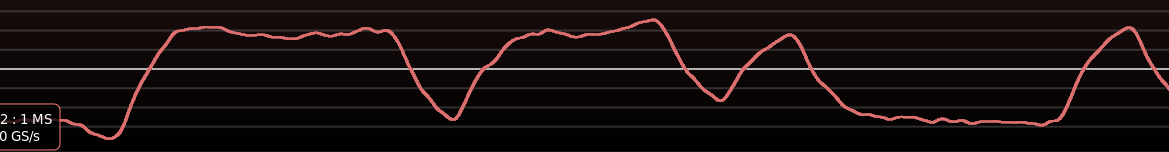
\includegraphics[width=10cm]{images/sparse-waveform.png}
\caption{Sparse waveform at a high zoom level}
\label{sparse-waveform}
\end{figure}

\begin{figure}[H]
\centering
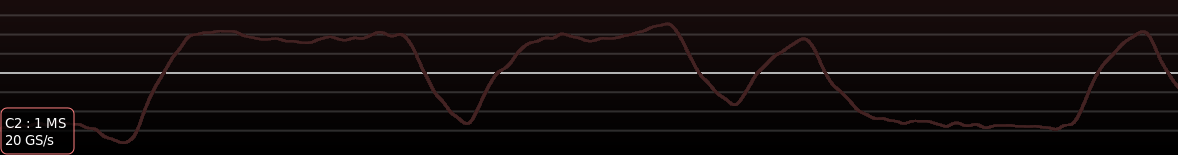
\includegraphics[width=10cm]{images/dim-waveform.png}
\caption{Dim waveform showing difficulty of seeing waveform at low opacity}
\label{dim-waveform}
\end{figure}

For example, the DVI waveform in Fig. \ref{washedout-waveform} looks like a solid white blob with a vaguely visible
outline. No fine detail can be observed other than the increased over/undershoot and random-looking edges on the
scanlines, compared to the flat appearance of the blanking period between scanlines and at the end of the frame.

When the opacity is reduced in this example, many more nuances of the signal become apparent. The high/low voltage
levels of the signal compared to the transitions between them are obvious, and the H/V sync pulses within the blanking
period show up as a slightly darker region.

\begin{figure}[H]
\centering
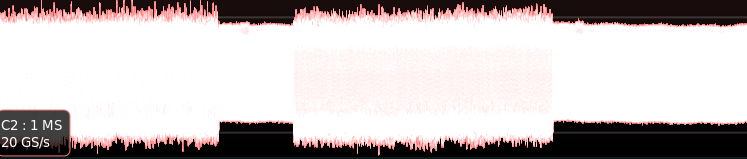
\includegraphics[width=10cm]{images/washedout-waveform.png}
\caption{Intensity-graded waveform showing washed-out appearance at high opacity}
\label{washedout-waveform}
\end{figure}

\begin{figure}[H]
\centering
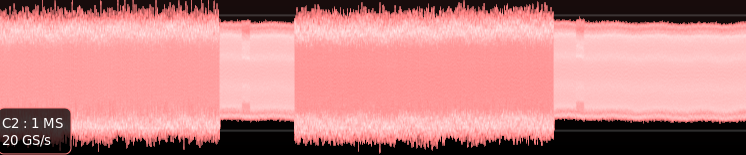
\includegraphics[width=10cm]{images/graded-waveform.png}
\caption{Intensity-graded waveform at lower opacity level}
\label{graded-waveform}
\end{figure}

As of this writing, the opacity setting is global for the entire application. Should this be changed to per waveform
group? If so, how should the group be selected and should there still be an option to make changes globally?
